\documentclass[letterpaper,12pt]{article}
\usepackage{apacite,pdfpages,enumitem,fancyhdr,url,graphicx,tabularx,ragged2e,booktabs,caption,epstopdf}
%http://www.ctan.org/tex-archive/biblio/bibtex/contrib/apacite/apacite.pdf
\usepackage[top=1in, bottom=1in, left=1in, right=1in]{geometry}
\usepackage[doublespacing]{setspace}
\pagestyle{fancy}
\setlist{nolistsep}
\setcounter{secnumdepth}{0}
\setlength{\skip\footins}{1.2cm}
\raggedbottom
\widowpenalty=1000
\clubpenalty=1000
\lhead{Reddit Pathways Paper}
\rhead{\thepage}
\cfoot{}
\title{Reddit Pathways Paper}
\begin{document}
\maketitle
\doublespacing

Reddit's subreddit-to-subreddit structure can be described as a directed, temporal network where nodes are subreddits, and edges are represented by the cumulative immediate consecutive posting history of users on the platform. For instance, if a user posts on subreddit A, and then posts on subreddit B, and then again on subreddit C, the posting history for this individual could be represented by a vector [A,B,C], where each consecutive pair of subreddits in this vector either create or add a weight of one to existing edges - in this case, two edges are generated from this posting history, A,B and B,C. These vectors of consecutive posting histories are generated for all users on Reddit, and are separated into daily summaries of activity across all subreddits. For example, the following graph would indicate that at the end of a day ($t=1$, where days are considered as timesteps), Reddit users who had immediately previously posted on subreddit A then posted on subreddit C 8 times, while users who had immediately previously posted on subreddit C then posted on subreddit A 3 times. For each of these nodes, the total number of times any individual started at that node and then posted on some other node is recorded. In this case, users transited a total of 38 times.

\begin{figure}[h]
  \centering
  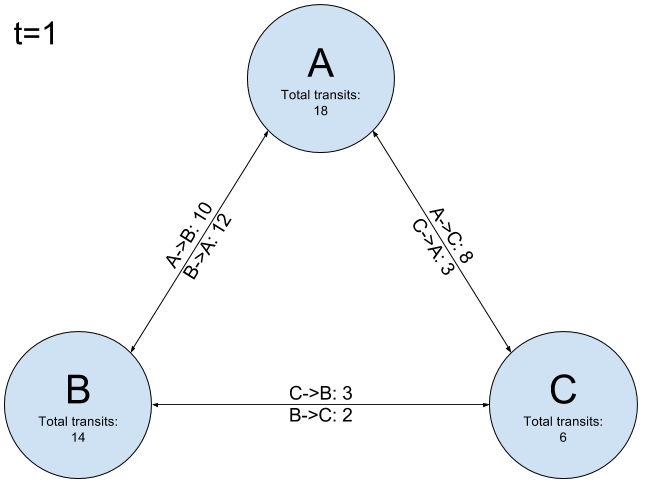
\includegraphics[width=\textwidth]{random_walk_ex}
  \caption{Example network.}
  \label{fig:random_walk_ex}
\end{figure}

This work seeks to describe the degree to which these transits differ from a parsimonious null model, namely the random walk. In a random walk model, the fraction of inbound walkers that a subreddit node $S_i$ receives from other subreddit nodes $S_j$ at some time $t$ is $\frac{1}{k(t)_j}$, where $k(t)_j$ is the number of other subreddits receiving walkers from node $S_j$ at $t$. In this case, the amount of traffic is moderated by the number of nodes that are connected to $S_j$ - if $S_j$ was tied to $k(t)_j = 100$ distinct nodes on a particular day (e.g. at least one person started at $S_j$ and then posted on some other $S_x \in S, S_x \neq S_j$), the expected fraction of walkers, or users posting on subreddits, that would next post on $S_j$ as opposed to all other directed neighbors of $S_j$ would be $\frac{1}{k(t)_j} = \frac{1}{100}$.

Following this intuition, then, it would be possible to compare the expected fraction provided by a random walk model against the observed fraction of nodes that actually did transit from $S_j$ to $S_i$ at $t$. We can define the observed number of walker paths transiting from $S_i$ to $S_j$ on a given day $t$ as $w_{ij}(t)$, which we can define as the error: 

$$e(S_i, S_j, t) = \sqrt{(\frac{1}{k(t)_j} - \frac{w_{ij}(t)}{\sum_k w_{jk}(t)})^2}$$

This can then be averaged across all inbound edges for $S_i$, which provides an estimate for how far the null expectation deviates from the observed fraction of walks that transit from $S_j$ to $S_i$: $ae(S_i, t) = \frac{\sum_j w_{ij}(t) e(S_i, S_j, t)}{\sum_j w_{ji}(t)}$. This weights the average appropriately, since some subreddits may send many walkers through, though the fractional deviance is relatively small, while others may send few walkers through, while the fractional deviance is very high.

This can then be summarized for an entire subreddit's history across all timesteps where $|t|$ denotes the total number of timesteps a subreddit was active on the platform (i.e. more than zero transits passed through the subreddit):

$$tae(S_i) = \frac{\sum_t ae(S_i, t)}{|t|}$$

This total average error can then be plotted against the total activity observed on the subreddit through the history of that subreddit - which provides the following chart:

\begin{figure}[h]
  \centering
  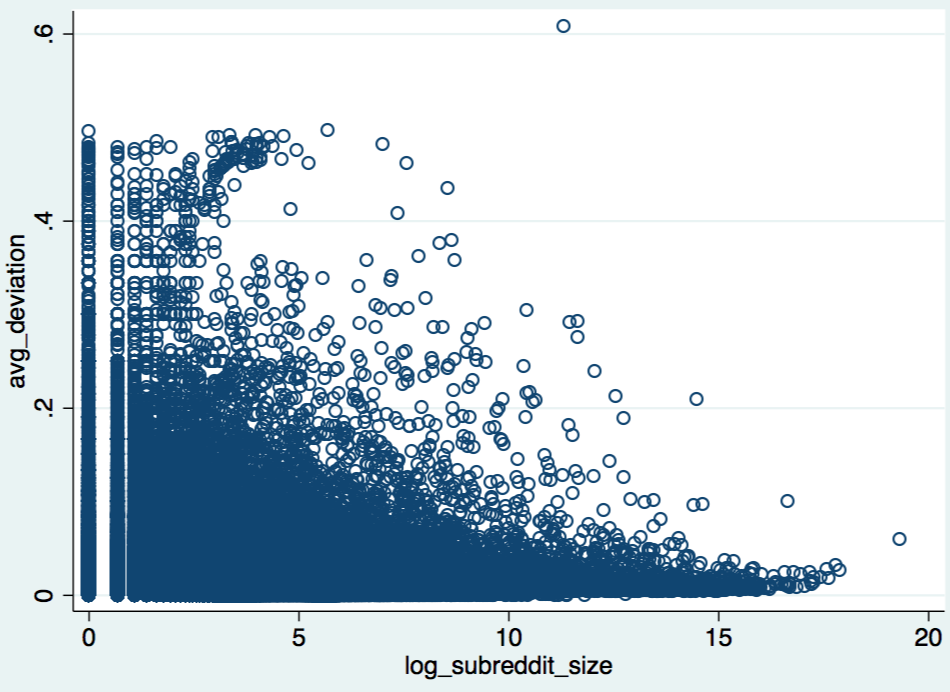
\includegraphics[width=\textwidth]{tae}
  \caption{Total average error for subreddits (y-axis) plotted by size of subreddit (x-axis)}
  \label{fig:tae}
\end{figure}
\clearpage
\end{document}